\section{Strategy to early predict potential failing students}

\label{sec:strategy}

Predicting the potential failing students early is very important in the sense that professors still have enough time to act and avoid students to fail the course. Notice that in case professors act based on the results of our strategy, we can indirectly help on reducing the high rate of failing students. However, in this article, we focus exclusively on identifying these students. This way, evaluating and reporting the rate after applying our strategy is outside the scope of this article.

Our strategy is automatic and consists of three simple steps: the use of a online judge system (Section~\ref{sec:online}), metrics collection (Section~\ref{sec:metrics}), and execution of a well-known clustering algorithm~\cite{hartigan-clustering-algorithms-1975} (Section~\ref{sec:clustering}).

Next, we detail the three steps of our strategy to predict the failing students.

\subsection{Online judge system}

\label{sec:online}

To assess the students performance during a course, it is important to closely monitor them. In this context, metrics represent an alternative to measure their performance. However, retrieving metrics regarding each student is a difficult and time-consuming task. To minimize this problem, one might rely on online learning tools, since these systems are not only a source for these metrics, but allow their automatic retrieval. 

A popular category of this kind of system is the online judges~\cite{uva, sphere}. Online judges provide a set of programming problems so that students can submit their solutions. After submitting, the online judge executes the solution against a set of predefined test cases. In case the solution passes over all the tests, the system evaluates the solution as correct. Otherwise, the system evaluates the solution according to the error type (e.g., wrong answer, compilation error, time limit exceeded, runtime error, etc) and even might give important tips so that students can successfully solve the problem afterwards.

Since students only learn how to program by programming~\cite{jenkins-ltsn02}, the online judge consists of an important environment in the sense students can constantly practice and improve their learning process. In addition, online judges play an important role regarding rapid, constructive, and corrective feedback, once professors are often overwhelmed with their daily activities\footnote{For instance, in Brazil professors very commonly deal with bureaucratic activities and have almost no support from administrative assistants.} and sometimes are not able to help each student separately~\cite{autolep-2011}. Supporting students is even harder in large class sizes~\cite{autolep-2011}, so an online tool helps on this front as well.

%Also, as the tool is available online, students can find their own rhythms.

Given all these advantages, the use of an online judge system is the first step of our strategy. We then can monitor students to automatically identify the candidates to fail the course.

\subsection{Metrics}

\label{sec:metrics}

The second step of our strategy consists of metrics retrieval. In particular, we retrieve two metrics by using the online judge system. We explain them in what follows:

\begin{itemize}

	\item \textbf{Number of submissions:} this metric represents the number of submissions a student does. Online judge systems commonly provide many problems. To solve a particular one, a student needs to submit at least one correct solution.

	\item \textbf{Number of correct submissions:} if a student solves one problem, we increase this metric by one.

\end{itemize}

Depending on the level of difficulty of a problem, students may submit solutions several times. However, notice that this is not necessarily bad regarding the learning process. For example, submitting many times means that students are somehow practicing and studying continuously. Thus, although she is not hitting a right solution, she is trying hard and will eventually hit one. Thus, the number of submissions metric is a good indicator of the amount of practice, which is very important in programming activities~\cite{cheang-online-judge-2003} and is frequently associated with the level of engaging and learning. However, when considered isolated, a high number of submissions may also mean that the student is getting frustrated due to so many wrong answers she receives. This way, we also consider the number of correct submissions to compensate and help us on studying such cases as well.

%\todo{Referencia do porque as metricas sao boas: quanto menos exercicio, maior a probabilidade de levar pau.}

\subsection{Clustering algorithm}

\label{sec:clustering}

To identify potential failing students, we use an existing clustering algorithm~\cite{hartigan-clustering-algorithms-1975} to define groups of students at the 30th day. Our idea consists of identifying different groups of students so we can clearly separate students likely to fail from the other ones. To compute the groups, the algorithm takes into account the metrics we present in Section~\ref{sec:metrics}. To make the strategy parameterizable in terms of number of groups, we use the well-known k-means~\cite{k-means-1979} clustering algorithm, which takes such a number as input.

Notice that the number of groups plays an important role on identifying potential failing students. In this article, we set the algorithm to compute two and three groups and evaluate both cases. For two groups, we have students who will either fail or pass. For three groups, we have fail, pass, and students that the strategy will not conclude anything about them, which we name ``inconclusive.'' This is reasonable since our study focuses on the very first 30 days, which means our drawings regarding the inconclusive group might be completely wrong: these students can either improve themselves and pass the course or fail due to several reasons.

We focus on two and three groups basically for two reasons: (i) using one group is useless; and (ii) more than three only brings more inconclusive groups to the table which, given our context, is pretty much the same of having only one inconclusive group.

\subsection{Summary}

%Figure~\ref{fig:strategy} combines all steps of our strategy. Notice that our

Our strategy is general in the sense we can use any online judge system, as long as it contains problems commonly found in introductory programming courses and we can collect the metrics we use from the system. In addition, notice that the strategy is automatic (no manual aptitude tests needed). This way, professors can apply the strategy more easily in their courses, reducing their effort.

To instantiate our strategy, we use the online judge system named \textit{Huxley}. The system is available online only in Portuguese\footnote{A video explaining Huxley with subtitles in english can be found at \url{bit.ly/huxleyvideo}} at \url{http://www.thehuxley.com/}. There are almost \huxleyProfessors registered professors and more than \huxleyCourses registered courses (all introductory in programming). Also, more than \huxleyInstitutions institutions around Brazil use the system. Huxley provides a database composed by more than \huxleyProblems problems classified according to level of difficulty and programming topics. This allows the students to choose the next problem in accordance to their corresponding levels. Notice that this helps on avoiding misleading in our metrics, e.g., many incorrect submissions to a problem that the student is not able to solve yet.

%and students are encouraged to use the system, once there is absolutely no penalty in case of wrong solutions.

%Huxley also classifies the problems according to level of difficulty and programming topics. This allows the students to choose the next problem in accordance to their corresponding levels.

%As the classes are happening, we encourage students to solve the problems available at Huxley. Although solving exercises is not mandatory, there are some particular activities where the professor forces students to use Huxley, such as formal exams.

%%%%%%%%%%%%%%%%%%%%%%%%%%%%%%%%%%%%%%%%%%%%%%%%%%%%%%%%%%%%%%%%%%%%%%%%%%%%%%
%This way, we let the students use the online judge during the very first 30 days (Step 1).
%%%%%%%%%%%%%%%%%%%%%%%%%%%%%%%%%%%%%%%%%%%%%%%%%%%%%%%%%%%%%%%%%%%%%%%%%%%%%%

Figure~\ref{fig:strategy} combines all steps of our strategy. We let the students use the online judge during the very first 30 days (Step 1), representing \semesterPercentage of the semester. At the end of the 30th day, the professor collects the metrics we detail in Section~\ref{sec:metrics} from the online judge system regarding the past 30 days (Step 2). Last but not least, the professor executes the k-means clustering algorithm (Step 3).

%To identify potential failing students \textit{early}, we collect the metrics for the first 30 days (representing \semesterPercentage of the semester) of the introductory programming courses. Then, we execute the k-means clustering algorithm.

\begin{figure}[h]
\centering
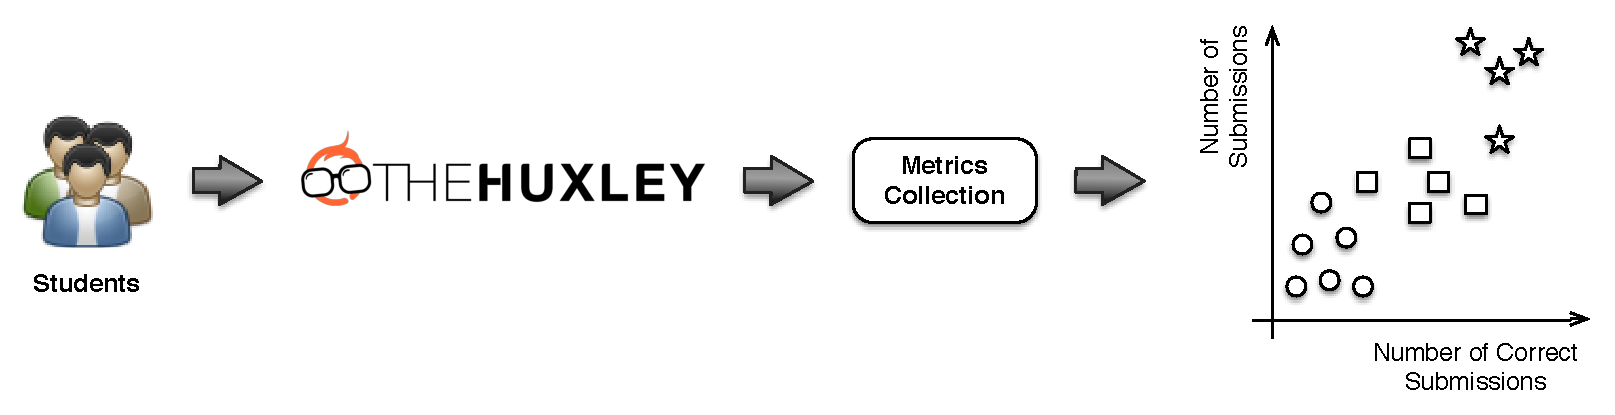
\includegraphics[width=1.0\textwidth,natwidth=610,natheight=642]{images/Strategy.pdf}
\caption{Summary of our strategy to identify potential failing students.}
\label{fig:strategy}
\end{figure}

We illustrate the k-means result in a two-dimensional plot (we represent one dimension for each metric we consider). Also, we illustrate the groups using shapes in Figure~\ref{fig:strategy}. In this particular case, we set k-means to compute three different groups. The circles represent the students candidates to fail the course. Notice that they submitted few solutions and few of them are correct.

%The same professor (Paes, one of the authors) taught the 7 semesters. The classes happened in a lab and some exercises available in Huxley were solved during the class. The professor strongly encouraged all students to submit solutions for the problems available in Huxley during extra-class activities, once there is absolutely no penalty in case of wrong submitted solutions. However, during the first 30 days, the use of Huxley was mandatory for approximately 6 exercises (used as a small percentage of the final grade) and for the first formal exam (held closely to the 30th day).

%\todo{Como deixar a estrategia mais geral? Dizer que pode ser qualquer online judge desde que tenha as metricas? Dizer que e mais geral e que instanciamos a estrategia com o huxley.}